\documentclass[../hw.tex]{subfiles}
\begin{document}
\setcounter{section}{5}
\begin{center}
  \section*{Homework 5} \label{sec:homework5}
  \subsection*{Due 2/21}
\end{center}
\addcontentsline{toc}{section}{\nameref{sec:homework5}}
\hrule \vspace{10px}

\paragraph*{1.} (a) If $f$ is independent of $y$, then 
\begin{align*}
    \pdv{f}{y} = 0
\end{align*}
and using the Euler-Lagrange (EQ) equation, we have
\begin{align*}
    \pdv{f}{y} - \dv{x}(\pdv{f}{y'}) = 0 \qor \pdv{f}{y} = \dv{x}(\pdv{f}{y'})
\end{align*}
so
\begin{align*}
    0 = \dv{x}(\pdv{f}{y'})
\end{align*}
and for the derivative to be zero,
\begin{align*}
    \pdv{f}{y'} = \mathrm{constant}
\end{align*}
(b) Since $f$ is independent of $x$,
\begin{align*}
    \pdv{f}{x} = 0
\end{align*}
Using the Euler-Lagrange equation, we have
\begin{align*}
    \pdv{f}{y} = \dv{x}(\pdv{f}{y'})
\end{align*}

Using chain rule to differentiate $f$ with respect to $x$ for a general function $f(x, y, y')$,
\begin{align*}
    \dv{x}f(x, y, y') &= \pdv{f}{x} \qt(\dv{x} x) + \pdv{f}{y} \qt(\dv{y}{x})
        + \pdv{f}{y'} \qt(\dv{y'}{x}) \\
    &= \pdv{f}{x} + \pdv{f}{y}y' + \pdv{f}{y'}y'' \\
    \dv{x}f(y, y') &= 0 + \pdv{f}{y}y' + \pdv{f}{y'}y''
\end{align*}
and substituting what we got from the EL equation,
\begin{align*}
    \dv{x}f(y, y') = \qt[\dv{x}(\pdv{f}{y'})]y' + \pdv{f}{y'} y'' = \qt[\dv{x}(\pdv{f}{y'})]y'
        + \pdv{f}{y'} \qt(\dv{y'}{x})
\end{align*}
which is equivalent to 
\begin{align*}
    \dv{x}f = \dv{x}(y' \pdv{f}{y'})
\end{align*}
from chain rule. Moving everything to one side:
\begin{align*}
    \dv{x}f - \dv{x}(y' \pdv{f}{y'}) &= 0 \\
    \dv{x}(f - y' \pdv{f}{y'}) &= 0
\end{align*}
which is only true if 
\begin{align*}
    f - y' \pdv{f}{y'} = \mathrm{constant}
\end{align*}

\newpage
\paragraph*{2.} (a) In 2D, we know the length of a short segment is
\begin{align*}
    \dd s = \sqrt{\dd x^2 + \dd y^2} 
\end{align*}
and in 3D
\begin{align*}
    \dd s = \sqrt{\dd x^2 + \dd y^2 + \dd z^2}
\end{align*}
transforming to spherical coordinates:
\begin{align*}
    x &= r\cos\phi \sin\theta \quad \dd x = \dd r \cos\phi \sin\theta
        - r \sin\phi \sin\theta \dd \phi + r \cos\phi \cos\theta \dd \theta \\
    y &= r\sin\phi \sin\theta \quad \dd y = \dd r \sin\phi \sin\theta
        + r \cos\phi \sin\theta \dd \phi + r \sin\phi \cos\theta \dd \theta \\
    z &= r\cos\theta \quad \dd z = \dd r \cos\theta - r \sin\theta \dd \theta
\end{align*}
for the sphere of radius $r \to R$ and $\dd r = 0$ since radius is constant, so
\begin{align*}
    \dd x &= - R \sin\phi \sin\theta \dd \phi + R \cos\phi \cos\theta \dd \theta \\
    \dd y &= R \cos\phi \sin\theta \dd \phi + R \sin\phi \cos\theta \dd \theta \\
    \dd z &= - R \sin\theta \dd \theta
\end{align*}
and squaring each term:
\begin{align*}
    \dd x^2 &= \color{draculacyan} R^2 \sin^2\phi \sin^2\theta \dd\phi^2
        \color{draculagreen} + R^2 \cos^2\phi \cos^2\theta \dd\theta^2
        \color{draculafg} - 2R^2 \sin\phi \sin\theta \cos\phi \cos\theta \dd\phi\dd\theta \\  
    \dd y^2 &= \color{draculacyan} R^2 \cos^2\phi \sin^2\theta \dd\phi^2
        \color{draculagreen} + R^2 \sin^2\phi \cos^2\theta \dd\theta^2
        \color{draculafg}+ 2R^2 \sin\phi \sin\theta \cos\phi \cos\theta \dd\phi\dd\theta \\
    \dd z^2 &= \color{draculagreen} R^2 \sin^2\theta \dd\theta^2
\end{align*}
when we add all three equations we can see that the last term in $\dd x^2$ and $\dd y^2$ cancel out,
and grouping the like terms we get
\begin{align*}
    \color{draculacyan} R^2 \sin^2\phi \sin^2\theta \dd\phi^2 + R^2 \cos^2\phi \sin^2\theta \dd\phi^2
        &= R^2 \sin^2\theta \dd\phi^2 (\sin^2\phi + \cos^2\phi) \\
        &= R^2 \sin^2\theta \dd\phi^2
\end{align*}
and 
\begin{align*}
    \color{draculagreen} R^2 \cos^2\phi \cos^2\theta \dd\theta^2
        & \color{draculagreen} + R^2 \sin^2\phi \cos^2\theta \dd\theta^2
        + R^2 \sin^2\theta \dd\theta^2 \\
        &= R^2 \cos^2\theta \dd\theta^2 (\cos^2\phi + \sin^2\phi) + R^2 \sin^2\theta \dd\theta^2 \\
        &= R^2 \dd\theta^2 (\cos^2\theta + \sin^2\theta)\\
        &= R^2 \dd\theta^2
\end{align*}
so the length of a short segment in spherical coordinates is
\begin{align*}
    \dd s &= \sqrt{R^2 \dd\theta^2 + R^2 \sin^2 \theta \dd\phi^2 } \\
        &= \sqrt{R^2 \dd\theta^2 \qt(\frac{\dd\theta^2}{\dd\theta^2}
            + \sin^2\theta \frac{\dd\phi^2}{\dd\theta^2})} \\
    \qusing &\dv{\phi}{\theta} = \phi'(\theta) \\
    &= R \sqrt{1 + \sin^2\theta \phi'(\theta)^2} \dd \theta 
\end{align*}
and the total path length $L$ is found by integrating $\dd s$ from $\theta_a$ to $\theta_b$: 
\begin{align*}
    L = R \int_{\theta_a}^{\theta_b} \sqrt{1 + \sin^2\theta \phi'(\theta)^2} \dd \theta
\end{align*}
(b) We find that the integral function is independent of $\phi$ or
\begin{align*}
    f = f(\theta, \phi') = \sqrt{1 + \sin^2\theta \phi'(\theta)^2}
\end{align*} so from 
Problem 1a, we know that
\begin{align*}
    \pdv{f}{\phi'} = \mathrm{constant} = C \\
    \pdv{f}{\phi'} = \frac{\sin^2\theta \phi'(\theta)}{\sqrt{1 + \sin^2\theta \phi'(\theta)^2}}
\end{align*}
setting one of the points to be the north pole, $\theta_a = 0$, so the constant is
\begin{align*}
    \frac{\sin^2(0) \phi'(0)}{\sqrt{1 + \sin^2(0) \phi'(0)^2}} = 0 = C
\end{align*}
solving for $\phi'(\theta)$
\begin{align*}
    \frac{\sin^2\theta \phi'(\theta)}{\sqrt{1 + \sin^2\theta \phi'(\theta)^2}} &= 0 \\
    \phi'(\theta) &= 0
\end{align*}
using separation of variables,
\begin{align*}
    \dv{\phi}{\theta} &= 0 \\
    \int \dd \phi &= \int 0 \dd \theta \\
    \phi(\theta) &= C_2
\end{align*}
Since $\phi$ is a constant, this is equivalent to to a slice of the sphere through the north pole,
which has a cross section of a circle with radius $R$. The path follows the circumference of the
circle, from the north pole to the point at $\theta_b$.

\newpage
\paragraph*{3.} (a) Finding the 2D length element in polar coordinates:
\begin{align*}
    x &= r\cos\phi \quad \dd x = \dd r \cos\phi - r\sin\phi \dd\phi \\
    y &= r\sin\phi \quad \dd y = \dd r \sin\phi + r\cos\phi \dd\phi
\end{align*}
so the length element is
\begin{align*}
    \dd x^2 + \dd y^2 &= (\dd r \cos\phi - r\sin\phi \dd\phi)^2
        + (\dd r \sin\phi + r\cos\phi \dd\phi)^2 \\
    &= \dd r^2 \cos^2\phi + r^2\sin^2\phi \dd\phi^2
        \color{draculapurple} - 2r\sin\phi \dd r \dd\phi \\
    &+ \dd r^2 \sin^2\phi + r^2\cos^2\phi \dd\phi^2 
        \color{draculapurple} + 2r\cos\phi \dd r \dd\phi \\
    &= \dd r^2 (\cos^2\phi+ \sin^2\phi) + r^2 \dd\phi^2 (\sin^2\phi + \cos^2\phi) \\
    &= \dd r^2 + r^2 \dd\phi^2
\end{align*}
so the length element in polar coordinates is
\begin{align*}
    \dd l = \sqrt{\dd r^2 + r^2 \dd\phi^2}
\end{align*}
and solving for $\dd\phi$,
\begin{align*}
    \dd l^2 &= \dd r^2 + r^2 \dd\phi^2 \\
    \dd\phi^2 &= \frac{\dd l^2 - \dd r^2}{r^2} \\
    \dd\phi &= \frac{1}{r} \sqrt{\dd l^2 - \dd r^2} \\
    \dd\phi &= \frac{1}{r} \sqrt{1 - \qt(\dv{r}{l})^2} \dd l
\end{align*}
plugging into the area integral:
\begin{align*}
    A &= \int_0^{2\pi} \frac{1}{2} r^2 \dd \phi \\
    &= \int_0^L \frac{1}{2} r^2 \qt[\frac{1}{r} \sqrt{1 - \qt(\dv{r}{l})^2} \dd l] \\
    &= \frac{1}{2} \int_0^L r \sqrt{1 - \qt(\dv{r}{l})^2} \dd l
\end{align*}
so the function in the integrand is
\begin{align*}
    f = f(r, r') = r \sqrt{1 - r'^2}
\end{align*}
(b) From Problem 1b we know that the conserved quantity we know that $f$ is independent of $l$, so
\begin{align*}
    f - r' \pdv{f}{r'} = \mathrm{constant} = K
\end{align*}
using the partial derivative
\begin{align*}
    \pdv{f}{r'} = \frac{r}{2\sqrt{1 - r'^2}} (-2r') = -\frac{r r'}{\sqrt{1 - r'^2}}
\end{align*}
So the conserved quantity is
\begin{align*}
    K &= r\sqrt{1 - r'^2} + \frac{r r'^2}{\sqrt{1 - r'^2}} \\
    &= \frac{r(1 - r'^2) + r r'^2}{\sqrt{1 - r'^2}} \\
    K &= \frac{r}{\sqrt{1 - r'^2}}
\end{align*}
rearranging for $r'$;
\begin{align*}
    K\sqrt{1 - r'^2} &= r \\
    K^2(1 - r'^2) &= r^2 \\
    K^2 - K^2 r'^2 &= r^2 \\
    K^2 r'^2 &= r^2 - K^2 \\
    r'^2 &= \frac{r^2}{K^2} - 1\\
    r' &= \sqrt{\frac{r^2}{K^2} - 1} = \dv{r}{l} 
\end{align*}
using separation of variables:
\begin{align*}
    \dd l &= \frac{\dd r}{\sqrt{r^2/K^2 - 1}} \\
\end{align*}
using the substitution $u = r/K$ and $\dd u = \dd r/K$:
\begin{align*}
    \dd l &= \frac{K \dd u}{\sqrt{u^2 - 1}} \\
    \int \dd l &= K \int \frac{\dd u}{\sqrt{u^2 - 1}} \\
    l &= K \arccosh(r/K) + C \\
    \arccosh(r/K) &= \frac{l - C}{K} \\
    r &= K \cosh\qt(\frac{l - C}{K})
\end{align*}
Since the constraint $l$ is constant as the total length of the curve ($K$ \& $C$ are also
constants), $r =$ constant is a solution to the equation or the radius of the curve is constant.
This is only true for circles which have a constant radial distance from the origin, so circles
leads to the maximum area integral. 
\newpage
\paragraph*{4.} (a) The kinetic energy of the particle is
\begin{align*}
    T = \frac{1}{2} m \vb v \cdot \vb v
        = \frac{1}{2} m (\dot r^2 + r^2 \dot\theta^2 + r^2 \dot \phi^2 \sin^2\theta )
\end{align*}
so the Lagrangian is
\begin{align*}
    \lagr = T - U = \frac{1}{2} m (\dot r^2 + r^2 \dot\theta^2 + r^2 \dot \phi^2 \sin^2\theta) - U
\end{align*}
where $U = U(r, \theta, \phi)$ and the Euler-Lagrange equations are
\begin{align*}
    \pdv{\lagr}{r} &= \dv{t}(\pdv{\lagr}{\dot r}) \\
    \pdv{\lagr}{\theta} &= \dv{t}(\pdv{\lagr}{\dot \theta}) \\
    \pdv{\lagr}{\phi} &= \dv{t}(\pdv{\lagr}{\dot \phi})
\end{align*}
For the first equation:
\begin{align*}
    \pdv{\lagr}{r} &= mr (\dot \theta^2 + \dot \phi^2 \sin^2\theta) - \pdv{r} U(r) \\
    \dv{t}(\pdv{\lagr}{\dot r}) &= \dv{t}(m \dot r) = m \ddot r
\end{align*}
so 
\begin{align*}
    m \ddot r &= mr (\dot \theta^2 + \dot \phi^2\sin^2\theta) - \pdv{U}{r} \\
    -\pdv{U}{r} &= m (\ddot r - r \dot \theta^2 - r \dot \phi^2 \sin^2\theta)
\end{align*}
For the second equation:
\begin{align*}
    \pdv{\lagr}{\theta} &= mr^2 \dot\phi^2 \sin\theta \cos\theta - \pdv{U}{\theta} \\
    \dv{t}(\pdv{\lagr}{\dot \theta}) &= \dv{t}(mr^2 \dot\theta) = m r^2 \ddot\theta + 2mr\dot r \dot\theta
\end{align*}
so 
\begin{align*}
    m r^2 \ddot\theta + 2mr \dot r \dot \theta &= mr^2 \dot\phi^2 \sin\theta \cos\theta - \pdv{U}{\theta} \\
    -\pdv{U}{\theta} &= m (r^2 \ddot\theta + 2r \dot r \dot \theta - r^2 \dot\phi^2 \sin\theta \cos\theta) \\
    - \frac{1}{r} \pdv{U}{\theta} &= m (r\ddot \theta + 2 \dot r \dot \theta - r \dot\phi^2 \sin\theta \cos\theta)
\end{align*}
and for the third equation:
\begin{align*}
    \pdv{\lagr}{\phi} &= - \pdv{U}{\phi} \\
    \dv{t}(\pdv{\lagr}{\dot \phi}) &= \dv{t}(mr^2 \dot\phi \sin^2\theta) \\
    &= 2mr \dot r \dot\phi\sin^2\theta + mr^2 \ddot\phi \sin^2\theta + 2mr^2 \dot\phi \dot\theta \sin\theta \cos\theta
\end{align*}
so 
\begin{align*}
    mr^2 \ddot \phi \sin^2 \theta &= - 2mr \dot r \dot\phi\sin^2\theta
        - 2mr^2 \dot\phi \dot\theta \sin\theta \cos\theta - \pdv{U}{\phi} \\
    - \pdv{U}{\phi} &= m(r^2 \ddot\phi \sin^2\theta + 2r \dot r \dot\phi\sin^2\theta
        + 2r^2 \dot\phi \dot\theta \sin\theta \cos\theta) \\
    - \frac{1}{r\sin\theta} \pdv{U}{\phi} &= m(r\ddot\phi \sin\theta + 2\dot r \dot\phi \sin\theta
         + 2r \dot\phi \dot\theta \cos\theta)
\end{align*}
where we have the 3 equations of motion:
\begin{align*}
    -\pdv{U}{r} &= m (\ddot r - r \dot \theta^2 - r \dot \phi^2 \sin^2\theta) \\
    - \frac{1}{r} \pdv{U}{\theta} &= m (r\ddot \theta + 2 \dot r \dot \theta - r \dot\phi^2 \sin\theta \cos\theta) \\
    - \frac{1}{r\sin\theta} \pdv{U}{\phi} &= m(r\ddot\phi \sin\theta + 2\dot r \dot\phi \sin\theta
         + 2r \dot\phi \dot\theta \cos\theta)
\end{align*}
where from N2L in spherical coordinates, the components of acceleration are
\begin{align*}
    a_r &=  \ddot r - r \dot \theta^2 - r \dot \phi^2 \sin^2\theta \\
    a_\theta &= r\ddot \theta + 2 \dot r \dot \theta - r \dot\phi^2 \sin\theta \cos\theta \\
    a_\phi &= r\ddot\phi \sin\theta + 2\dot r \dot\phi \sin\theta
         + 2r \dot\phi \dot\theta \cos\theta
\end{align*}
and the conservative force is 
\begin{align*}
    \vb F = -\grad U = -\pdv{U}{r} \vu r - \frac{1}{r} \pdv{U}{\theta} \vu \theta - \frac{1}{r\sin\theta} \pdv{U}{\phi} \vu \phi   
\end{align*}
To compare with N2L we start with the unit vectors in spherical coordinates:
\begin{align*}
    \vu r &= \sin\theta \cos\phi \vu x + \sin\theta \sin\phi \vu y + \cos\theta \vu z \\
    \vu \theta &= \cos\theta \cos\phi \vu x + \cos\theta \sin\phi \vu y - \sin\theta \vu z \\
    \vu \phi &= -\sin\phi \vu x + \cos\phi \vu y
\end{align*}
and from the velocity equation we know that the derivative of the radial unit vector is
\begin{align*}
    \dot{\vu r} = \dot \theta \vu* \theta + \dot \phi \sin\theta \vu* \phi
\end{align*}
for the colatitude unit vector in the $\theta$ direction
\begin{align*}
    \dot{\vu* \theta} &= (-\dot\theta \sin\theta \cos\phi  -\dot \phi \cos\theta \sin\phi) \vu x +
        (-\dot\theta \sin\theta \sin\phi + \dot \phi \cos\theta \cos\phi) \vu y 
        - \dot\theta \cos\theta \vu z \\
        &= \dot\phi \cos\theta \vu* \phi - \dot\theta \vu r
\end{align*}
(linear combination of unit vectors) and for the azimuthal unit vector in the $\phi$ direction
\begin{align*}
    \dot{\vu*\phi} &= -\dot\phi \sin\phi \vu x - \dot\phi \cos\phi \vu y \\
    &= -\dot\phi \sin\theta \vu r - \dot\phi \cos\theta \vu* \theta
\end{align*}
with this in hand taking the time derivative of velocity:
\begin{align*}
    \dv{t} \vb v &= \dv{t} (\dot r \vu r + r \dot \theta \vu \theta + r \dot \phi \sin\theta \vu \phi) \\
\end{align*}
the first term is
\begin{align*}
    \dv{t} (\dot r \vu r) &= \ddot r \vu r + \dot r \dot{\vu r} \\
    &= \ddot r \vu r + \dot r \dot \theta \vu* \theta + \dot r \dot \phi \sin\theta \vu* \phi
\end{align*}
the second term is
\begin{align*}
    \dv{t} (r \dot \theta \vu \theta) &= (\dot r \dot\theta + r \ddot \theta) \vu*\theta
        + r\dot\theta(\dot\phi \cos\theta \vu* \phi - \dot\theta \vu r) \\
    &= (-r\dot\theta^2) \vu r + (\dot r \ddot \theta) \vu*\theta
        + (r \dot\phi \dot\theta \cos\theta) \vu*\phi
\end{align*}
and the third term is
\begin{align*}
    \dv{t} (r \dot \phi \sin\theta \vu*\phi) &=
        (\dot r \dot\phi \sin\theta + r\ddot\phi \sin\theta + r \dot\phi \dot\theta \cos\theta) \vu*\phi
        + r\dot\phi \sin\theta (-\dot\phi \sin\theta \vu r - \dot\phi \cos\theta \vu*\theta) \\
    &= (-r\dot\phi^2 \sin^2\theta) \vu r 
        + (-r\dot\phi^2\sin\theta\cos\theta) \vu*\theta
        + (\dot r \dot\phi \sin\theta + r\ddot\phi\sin\theta + r \dot\phi \dot\theta \cos\theta) \vu*\phi
\end{align*}
so combing all the terms:
\begin{align*}
    \dv{t} \vb v &= (\ddot r - r\dot\theta^2 - r\dot\phi^2\sin^2\theta) \vu r
        + (r\ddot\theta + 2\dot r \dot\theta - r\dot\phi^2\sin\theta\cos\theta) \vu*\theta \\
        &+ (r\ddot\phi\sin\theta + 2\dot r \dot\phi\sin\theta + 2r\dot\phi\dot\theta\cos\theta) \vu*\phi
\end{align*}

\newpage
\paragraph*{5.} (a) 
In the frame where the cart is at rest at $x' = x - v_o t$ this is simply the Brachistochrone
where the time of travel is 
\begin{align*}
    T = \int_A^B \frac{\dd s}{v}
\end{align*}
and the short segment length is
\begin{align*}
    \dd s = \sqrt{\dd x'^2 + \dd y^2} = \sqrt{1 + \qt(\dv{y}{x'})^2} \dd x' \qor \sqrt{1 + y'^2} \dd x
\end{align*}
and from the conservation of energy
\begin{align*}
    \frac{1}{2} m v^2 = mgy \qor v = \sqrt{2gy}
\end{align*}
so
\begin{align*}
    T = \int_A^B \frac{\sqrt{1 + y'^2}}{\sqrt{2gy}} \dd x'
\end{align*}
where the integral function is independent of $x$;
\begin{align*}
    f = f(y, y') = \frac{\sqrt{1 + y'^2}}{\sqrt{2gy}}
\end{align*} so using the second form of 
the EL equation from Problem 1b, we have
\begin{align*}
    f - y' \pdv{f}{y'} = \mathrm{constant} = C
\end{align*}
using using the partial derivative
\begin{align*}
    \pdv{f}{y'} = \frac{1}{\sqrt{2gy}} \frac{y'}{\sqrt{1 + y'^2}}
\end{align*}
so the conserved quantity is
\begin{align*}
    C &= \frac{\sqrt{1 + y'^2}}{\sqrt{2gy}} - \frac{y'}{\sqrt{2gy}\sqrt{1 + y'^2}} \\
    &= \frac{1}{\sqrt{2gy}\sqrt{1 + y'^2}}
        \qt[\frac{\cancel{\sqrt{2gy}} \sqrt{1 + y'^2} \sqrt{1 + y'^2}}{\cancel{\sqrt{2gy}}}
        - y'^2] \\
    &= \frac{1}{\sqrt{2gy}\sqrt{1 + y'^2}} \\
    \qor 2C^2g &= \frac{1}{y(1 + y'^2)}
\end{align*}
setting a new constant 
\begin{align*}
    2C^2 g = \frac{1}{2a} \qqtext{where} C = \sqrt{\frac{1}{4ga}}
\end{align*}
we can now solve for $y'$:
\begin{align*}
    \frac{1}{2a} &= \frac{1}{y(1 + y'^2)} \\
    1 + y'^2 &= \frac{2a}{y} \\
    y'^2 &= \frac{2a}{y} - 1 \\
    y' &= \sqrt{\frac{2a}{y} - 1} \qor \sqrt{\frac{2a - y}{y}}
\end{align*}
using separation of variables:
\begin{align*}
    \dv{y}{x'} &= \sqrt{\frac{2a - y}{y}} \\
    \int \dd y \sqrt{\frac{y}{2a - y}}  &= \int \dd x'
\end{align*}
and using the substitution $y = a(1 - \cos\theta);\quad \dd y = \dd \theta a\sin\theta $ and
\begin{align*}
    \sin^2\theta &= 1 - \cos^2\theta \\
    \sin\theta &= \sqrt{1 - \cos^2\theta} = \sqrt{1 - \cos\theta} \sqrt{1 + \cos\theta}
\end{align*}
so 
\begin{align*}
    x' &= \int \dd \theta a \sin\theta \sqrt{\frac{a(1 - \cos\theta)}{2a - a(1 - \cos\theta)}} \\
    &= \int \dd \theta a \sqrt{1 - \cos\theta} \cancel{\sqrt{1 + \cos\theta}}
      \frac{\sqrt{1 - \cos\theta}}{\cancel{\sqrt{1 + \cos\theta}}} \\
    &= a \int \dd \theta (1 - \cos\theta) = a (\theta - \sin\theta)
\end{align*}
since the $\theta = \omega t$ we have the parametric equation for the path in the reference frame
\begin{align*}
    x'(t) &= a(\omega t - \sin(\omega t)) \\
    y(t) &= a(1 - \cos(\omega t))
\end{align*}
since $x = x' + v_o t$ the $x$ position in the original frame is
\begin{align*}
    x(t) &= a(\omega t - \sin(\omega t)) + v_o t
\end{align*}
(b) Using the initial conditions
\begin{align*}
    x = y = 0, \; \dot x = v_o, \; \dot y = 0
\end{align*}
we first solve for $\omega$:
\begin{align*}
    \dot x &= a\omega(1 - \cos(\omega t)) + v_o \\
    \dot y &= a\omega\sin(\omega t)
\end{align*}
we know at $t = 0$ that $\dot x = v_o$ and $\dot y = 0$. Since $\ddot y = g$ from the gravitational
force we can solve for $\omega$:
\begin{align*}
    \ddot y(t) &= a\omega^2\cos(\omega t) \\
    \ddot y(0) &= a\omega^2 = g \implies \omega = \sqrt{\frac{g}{a}}
\end{align*}
At the boundary point $B$ we know that the cycloid completes one cycle so $\omega t = 2\pi$:
\begin{align*}
    x'(t_B) &= a(2\pi - \sin(2\pi)) = L \\
    L &= 2\pi a \implies a = \frac{L}{2\pi} \implies \omega = \sqrt{\frac{2\pi g}{L}}
\end{align*}
so 
\begin{align*}
    x(t) &= \frac{L}{2\pi} \qt[\sqrt{\frac{2\pi g}{L}} t - \sin(\sqrt{\frac{2\pi g}{L}} t)] 
    + v_o t \\
    y(t) &= \frac{L}{2\pi} \qt[1 - \cos(\sqrt{\frac{2\pi g}{L}} t)]
\end{align*}
\newpage
(c) Sketching the path
\begin{figure}[ht]
    \centering
    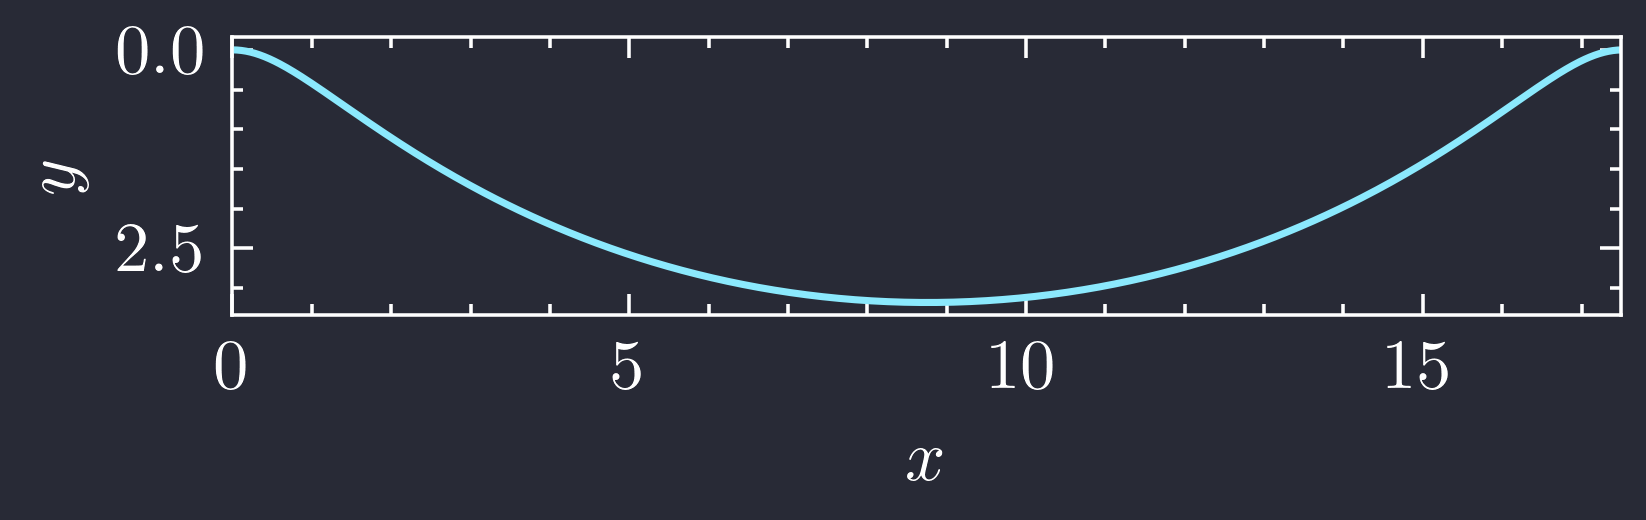
\includegraphics[width=0.8\linewidth]{hw5b.png}
    \caption{Numerically computed track shape}
\end{figure}

\end{document}